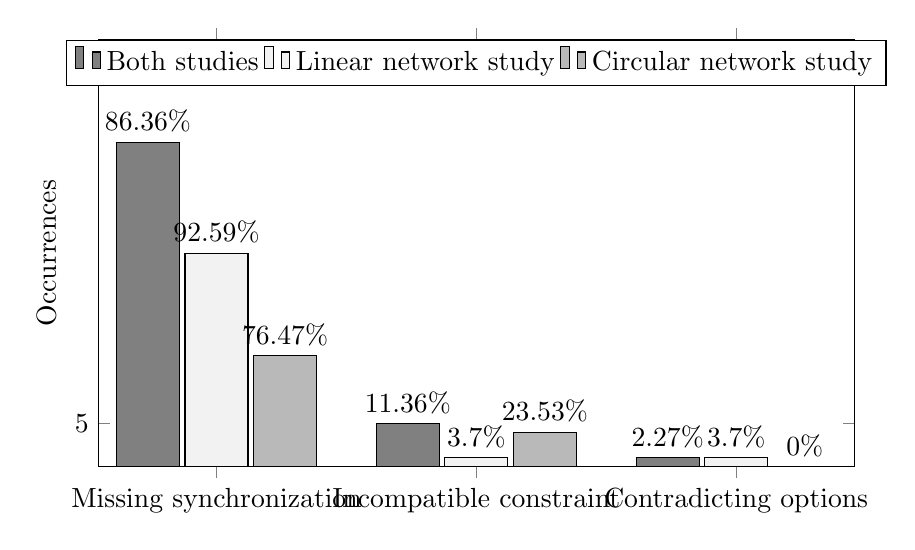
\begin{tikzpicture}
    \begin{axis}[
        ybar,
        bar width=0.8cm,
        x=3.3cm,
        height=7cm,
        legend style={at={(0.5,1)},anchor=north,legend columns=-1},
        ylabel={Occurrences},
        symbolic x coords={Missing synchronization, Incompatible constraint, Contradicting options},
        xtick=data,
        ytick=5,
        ymin=0,
        ymax=50,
        enlarge x limits={abs=1.5cm},
        nodes near coords align={vertical},
    ]
    \addplot[fill=gray,
        point meta={y*100/44}, % 44 Mistakes in total, calculate percentage
        nodes near coords={\pgfmathprintnumber\pgfplotspointmeta\%},
        ] table[x=Mistake type, y=occurrences, col sep=comma] {
            Mistake type,              occurrences
            Missing synchronization,   38
            Incompatible constraint,   5
            Contradicting options,     1
        };
    \addplot[fill=gray!10,
        point meta={y*100/27}, % 44 Mistakes in total, calculate percentage
        nodes near coords={\pgfmathprintnumber\pgfplotspointmeta\%},
        ] table[x=Mistake type, y=occurrences, col sep=comma] {
            Mistake type,              occurrences
            Missing synchronization,   25
            Incompatible constraint,   1
            Contradicting options,     1
        };
    \addplot[fill=gray!55,
        point meta={y*100/17}, % 17 Mistakes in total, calculate percentage
        nodes near coords={\pgfmathprintnumber\pgfplotspointmeta\%},
        ] table[x=Mistake type, y=occurrences, col sep=comma] {
            Mistake type,               occurrences
            Missing synchronization,    13
            Incompatible constraint,    4
            Contradicting options,      0
        };
        \legend{Both studies, Linear network study, Circular network study}
    \end{axis}
\end{tikzpicture}